\documentclass[a4paper]{paper}

\usepackage[utf8]{inputenc}
\usepackage{amsmath}
\usepackage[left=2.5cm,top=3cm,right=2.5cm,bottom=3cm,bindingoffset=0.cm]{geometry}
\usepackage{bm} % used for bold math symbols
\usepackage{parskip} % vertical space instead of indented paragraphs
\usepackage{hyperref}
\usepackage{graphicx}

\author{
Patrick Spieler \\
\texttt{stapelzeiger@gmail.com}
}

\title{Rotations \& Reference Frames}

\begin{document}
\maketitle
\hrule
\bigskip


\begin{abstract}

This document defines the reference frames and rotation conventions.

\end{abstract}

\tableofcontents

\pagebreak

\section{Reference Frames}

\subsection{Aircraft Geometric Frame}

The aircraft geometric frame $(x_a, y_a, z_a)$ is used to locate points in the aircraft.
It is fixed to the aircraft geometry, unlike the body frame, which is fixed to the centre of mass and can therefore depend on aircraft configuration.

The $x_a$ axis points backward, $y_a$ points right and $z_a$ points up.
The origin $O_a$ is located in the plane of right/left symmetry, at the nose tip (unless specified differently for a specific aircraft). See figure \ref{fig:aircraft_frame}.

The centre of mass, inertia tensor as well as the position of all the aircraft subsystems are to be specified in the aircraft frame.

\begin{figure}[h]
\centering
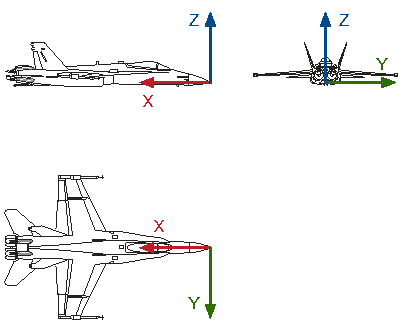
\includegraphics[width=0.4\textwidth]{img/aircraft_frame.pdf}
\caption{Aircraft frame, base image source: F-18 HARV from Dryden Flight Research Center Graphics Collection: https://www.dfrc.nasa.gov/Gallery/Graphics/index.html}
\label{fig:aircraft_frame}
\end{figure}

\subsection{Body Frame}

% todo forward, right should be more clear to avoid confusion with velocity direction
The body frame is used for dynamics computation of the aircraft.
The body reference frame $(x_b, y_b, z_b)$ rotates with the aircraft.
The $x_b$ axis points forward, $y_b$ points right and $z_b$ points down as shown in figure \ref{fig:body_frame}.
The origin $O_b$ of the aircraft coordinate system is fixed at the centre of mass.

\begin{figure}[h]
\centering
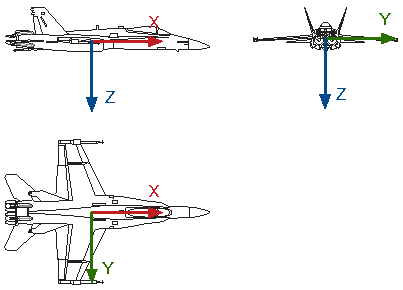
\includegraphics[width=0.4\textwidth]{img/body_frame.pdf}
\caption{Body frame, base image source: F-18 HARV from Dryden Flight Research Center Graphics Collection: https://www.dfrc.nasa.gov/Gallery/Graphics/index.html}
\label{fig:body_frame}
\end{figure}

\subsection{Inertial Frame}

The inertial frame used is fixed to the Earth surface and is therefore only an approximation of a true inertial reference frame.
Furthermore the gravity vector is assumed to be constant and pointing down.

The $(x_I, y_I, z_I)$ axes are chosen to be aligned with the true north, east and down (NED) direction respectively.
The origin $O_I$ is defined as the point of system initialization unless specified differently for the mission.



\section{Rotation Representation}

Rotations are used to define the relative orientation between two reference frames.
There are many different conventions for representing rotations, which is why it is important to clearly define which one is used.

The following definitions follow the active interpretation of rotation angles, meaning that the rotations specifies how the vectors/points are transformed. For more details about active vs passive conventions refer to section \ref{sec:actvie_vs_passive}.

\subsection{Rotation Matrix}

Rotation matrices are a convenient form to represent rotations and are computationally efficient in transforming vectors.

The rotation matrices around the three base vectors $\bm{x}$, $\bm{y}$ and $\bm{z}$ by an angle $\theta$ are given by:

\begin{equation}
\begin{split}
    R(\bm{x}, \theta) =
    \left[\begin{matrix}1 & 0 & 0\\
    0 & \cos{\left (\theta \right )} & - \sin{\left (\theta \right )}\\
    0 & \sin{\left (\theta \right )} & \cos{\left (\theta \right )}\end{matrix}\right]\\
    R(\bm{y}, \theta) =
    \left[\begin{matrix}\cos{\left (\theta \right )} & 0 & \sin{\left (\theta \right )}\\
    0 & 1 & 0\\
    - \sin{\left (\theta \right )} & 0 & \cos{\left (\theta \right )}\end{matrix}\right]\\
    R(\bm{z}, \theta) =
    \left[\begin{matrix}\cos{\left (\theta \right )} & - \sin{\left (\theta \right )} & 0\\
    \sin{\left (\theta \right )} & \cos{\left (\theta \right )} & 0\\
    0 & 0 & 1\end{matrix}\right]\\
\end{split}
\end{equation}


A rotation matrix for an arbitrary rotation axis is given by:

\begin{equation}
    todo
    \label{eq:rotation_matrix_angle_axis}
\end{equation}

A vector is rotated by a matrix using:


\begin{equation}
    \bm{v}' = R(\bm{n}, \theta) \bm{v}
\end{equation}


Rotations are chained following matrix multiplication rules. For example a rotation around y followed by a rotation around x is given by:

\begin{equation}
    \bm{v}' = R(\bm{x}, \theta_2) R(\bm{y}, \theta_1) \bm{v}
\end{equation}

\subsection{Quaternion}

Rotation Quaternions are a very efficient, non-singular rotation representation.
They require few operations to compose rotations and they use, with four components, the minimal amount of storage for a non-singular rotation representation.
Quaternions are thus a good choice for a general purpose rotation representation.

The quaternions are a number system that extends the complex numbers by two additional imaginary units. The following identity defines the quaternion algebra.

\begin{equation}
    i^2 = j^2 = k^2 = ijk = -1
\end{equation}

From this identity all products of the imaginary units can be derived. Note that the quaternion multiplication non-commutative.

For our application of quaternions to rotations it is practical to represent the quaternion as a four dimensional vector. We define the vector representation of the quaternion $q_0 + q_1 i + q_2 j + q_3 k$ as:
\begin{equation}
    q = q_0 + q_1 i + q_2 j + q_3 k = \left[ \begin{array}{c} q_0 \\ q_1 \\ q_2 \\ q_3  \end{array} \right]
\end{equation}
The three imaginary components can be combined to a vector $\bm{q}_v$.
\begin{equation}
    q = \left[ \begin{array}{c} q_0 \\ \bm{q}_v  \end{array} \right]
\end{equation}
In this form the multiplication between quaternions can be expressed in an elegant way using vector operations.
\begin{equation}
    p \circ q =
    \left[ \begin{array}{c} p_0 \\ \bm{p} \end{array} \right]
    \circ
    \left[ \begin{array}{c} q_0 \\ \bm{q} \end{array} \right]
    = \left[ \begin{array}{c}
            p_0 q_0 - \bm{p} \cdot \bm{q} \\
            p_0 \bm{q} + q_0 \bm{p} + \bm{p} \times \bm{q}
      \end{array} \right]
\label{eq:quat_mult_vect}
\end{equation}

\subsubsection{Rotation Quaternion}

A quaternion representing a rotation of $\theta$ around an axis $\bm{n}$ is given by:
\begin{equation}
    q(\bm n, \theta) =
        \left[\begin{array}{c}
            \cos{(\frac{\theta}{2})}\\
            \bm{n} \sin{(\frac{\theta}{2})}\\
        \end{array}\right]
\label{eq:rotation_quat}
\end{equation}
Such a rotation quaternion always has unit norm.
Note that $q$ and $-q$ represent the same rotation.
The convention is to choose $q_0$ positive.
The four components of a rotation quaternion are sometimes called Euler-Rodrigues parameters.

The rotation of a vector $\bm{v}$ by a unit quaternion is given by:
\begin{equation}
    \bar{\bm{v}}' = q \circ \bar{\bm{v}} \circ q^*
\label{eq:quat_rot_vect}
\end{equation}
Where $\bar{\bm{v}}$ is the quaternion with real part zero and vector part equal to $\bm{v}$
and $q^*$ is the conjugate of $q$ defined as:
\begin{equation}
    q^* = \left[ \begin{array}{c} q_0 \\ -q_1 \\ -q_2 \\ -q_3  \end{array} \right]
\end{equation}

From equation (\ref{eq:quat_rot_vect}) we find that chaining rotations can be achieved by quaternion multiplication. The rotation by $p \circ q$ is equivalent to the rotation by $q$, followed by the rotation by $p$. This is analogous to rotation matrix chaining.

A rotation matrix can be constructed from the rotation quaternion using the following formula:
\begin{equation}
    R(q) =
    \left[\begin{matrix}
    q_{0}^{2} + q_{1}^{2} - q_{2}^{2} - q_{3}^{2} &
        - 2 q_{0} q_{3} + 2 q_{1} q_{2} &
        2 q_{0} q_{2} + 2 q_{1} q_{3}\\
    2 q_{0} q_{3} + 2 q_{1} q_{2} &
        q_{0}^{2} - q_{1}^{2} + q_{2}^{2} - q_{3}^{2} &
        - 2 q_{0} q_{1} + 2 q_{2} q_{3}\\
    - 2 q_{0} q_{2} + 2 q_{1} q_{3} &
        2 q_{0} q_{1} + 2 q_{2} q_{3} &
        q_{0}^{2} - q_{1}^{2} - q_{2}^{2} + q_{3}^{2}
    \end{matrix}\right]
\end{equation}

An alternative notation of the rotation matrix of a quaternion using vector operations is:
\begin{equation}
R(q) = (q_0^2 - \lVert\bm{q}\rVert^2) I_{3x3} + 2 \bm{q} \bm{q}^T + 2 q_0 [\bm{q}]_{\times}
\label{eq:rotation_matrix_from_quaternion}
\end{equation}

where $[\bm{q}]_{\times}$ is the cross product matrix of $\bm{q}$ defined as:
\begin{equation}
    [\bm{q}]_{\times} = \left[
    \begin{matrix}
           0 & -q_3 &  q_2 \\
         q_3 &    0 & -q_1 \\
        -q_2 &  q_1 &    0 \\
    \end{matrix}
    \right]
\end{equation}



\section{Reference Frame Transformations}

The relative position and orientation between two reference frames are described by rotations and translation transformations of vectors represented in the two frames.

\subsection{Active vs. Passive Transformation Convention}
\label{sec:actvie_vs_passive}

There are two ways to define the relative orientation of two reference frames by means of rotation angles.
These are the active (alibi) and passive (alias) convention.
They are equivalent but differ in the interpretation of a rotation angle.

In the \textbf{active} convention, a rotation angle specifies how \textbf{vectors} in the reference frame are rotated when changing from the initial to the final frame.

In the \textbf{passive} convention, the rotation angle specifies how the coordinate \textbf{frame axes} are rotated. As a result, the passive description of the same transformation has the inverse sign of the angle compared to the active description. Furthermore, if a sequence of sequence of rotations (like Euler angles) are specified in the passive description, the corresponding active sequence is in reverse order and with the inverse sign.

The active description is used in geometry and commonly in robotics whereas the passive description is used commonly in aerospace.
Unfortunately the common definition of quaternion rotation representation in the passive convention differs from the active definition significantly.
In the passive convention the quaternion for a rotation about a certain angle is constructed the same way as for an angle in the active convention, but the rotation of a vector by a quaternion is defined differently. This can be seen in the following definition for a vector rotated by a quaternion:

\begin{align}
    \bar{\bm{v}}' = q \circ \bar{\bm{v}} \circ q^* && \textit{common definition in \textbf{active} convention.}\\
    \bar{\bm{v}}' = q^* \circ \bar{\bm{v}} \circ q && \textit{common definition in \textbf{passive} convention.}
\end{align}

From this definition follows, that the chaining rules for the passive convention are inverse to the the active one. The chaining order of the passive convention therefore no longer follows the order of matrix chaining, which lead some authors \cite{markley_quaternion} even to redefine the quaternion product to fix this.

A much simpler approach is to change only the construction of a quaternion for the passive angle convention. A quaternion from a passive rotation description would therefore be constructed with a negative sign in front of the angle and the rest of the quaternion algebra would follow the same equations as the active convention used in geometry.

The same problem is not existing for rotation matrices, where, in the passive description, the sign of the angle is reversed when constructing a rotation matrix and the matrix/vector algebra stays the same.

\subsubsection{Convention Used}

In terms of quaternion algebra, the convention that is chosen follows the \textbf{standard quaternions from math/geometry}. This corresponds to the same definition as used in the active convention.
The reason for this choice is the more consistent multiplication order when chaining rotations and the compatibility with existing geometry libraries.

However, the chosen standard interpretation of an angle that describes an attitude is the \textbf{passive} one, meaning that the angle describes how the reference frame is rotated.
The reason for this choice is that it is simpler to visualize passive transformation angles, especially when using Euler angles rotation sequences.

Note that in most parts of the code the choice of convention is irrelevant, as usually transformations like quaternions / matrices are used and the angle is not used directly for any computation.
In functions that take angles and where the convention is not obvious (like for example the construction of a rotation matrix from an axis/angle) the convention has to be documented explicitly, ideally in the name of the angle variable.
The place where the choice of convention matters mostly is when displaying attitude angles to a user.

As the quaternion algebra follows the active convention, a quaternion is constructed from an angle in the passive convention as follows: (notice the negative sign in front of the angle)

\begin{equation}
    q_{passive}(\bm n, \theta_{passive}) =
        \left[\begin{array}{c}
            \cos{(\frac{-\theta_{passive}}{2})}\\
            \bm{n} \sin{(\frac{-\theta_{passive}}{2})}\\
        \end{array}\right]
\end{equation}



\subsection{Reference Frame Notation}


Superscripts are used to denote the reference frame in which a vector is expressed.

$\bm{r}^k$ is the vector $\bm{r}$ expressed in the k-frame.

The transformation from the k-frame to the m-frame is given by:

\begin{equation}
    \bm{r}^m = R_k^m \bm{r}^k
\end{equation}

$R_k^m$ is the matrix that transforms a vector in the k-frame ($\bm{k}_x, \bm{k}_y, \bm{k}_z$) to a vector in the m-frame.

The matrix $R_k^m$ is composed of the base vectors of the k-frame expressed in the m-frame.

\begin{equation}
    R_k^m = \left[ \bm{k}_x^m, \bm{k}_y^m, \bm{k}_z^m \right]
\end{equation}

$\omega^i_{jk}$ is the rotational velocity of k relative to j expressed in i.

\subsection{Attitude Transformation}

\subsubsection{Matrix}

A rotation matrix representing the attitude transformation from frame $a$ to $b$ is constructed using equation \ref{eq:rotation_matrix_angle_axis}.
If the angle is in the angle represents the rotation of coordinate frame (passive convention):
\begin{equation}
    R_a^b = R_{passive}(\bm{n}, \theta^{passive}_{a \rightarrow b}) = R(\bm{n}, -\theta^{passive}_{a \rightarrow b})
\end{equation}
If the angle is in the angle represents the rotation of the points (active convention):
\begin{equation}
    R_a^b = R_{active}(\bm{n}, \theta^{active}_{a \rightarrow b}) = R(\bm{n}, \theta^{active}_{a \rightarrow b})
\end{equation}


\subsubsection{Quaternion}

A quaternion representing the attitude transformation from frame $a$ to $b$ is constructed using equation \ref{eq:rotation_quat}.
If the angle is in the angle represents the rotation of coordinate frame (passive convention):
\begin{equation}
    q_a^b = q_{passive}(\bm n, \theta^{passive}_{a \rightarrow b}) = q(\bm n, -\theta^{passive}_{a \rightarrow b})
\end{equation}
If the angle is in the angle represents the rotation of the points (active convention):
\begin{equation}
    q_a^b = q_{active}(\bm n, \theta^{active}_{a \rightarrow b}) =  q(\bm n, \theta^{active}_{a \rightarrow b})
\end{equation}

To transform vectors/points with the attitude quaternion equation \ref{eq:quat_rot_vect} can be used or alternatively if multiple points are transformed a rotation matrix can be constructed using equation \ref{eq:rotation_matrix_from_quaternion}.

\subsubsection{Euler Angles}

Euler angles are useful as a user interface, since they can be easily visualized and contain the minimal number of parameters. However, they are to be avoided for computation as they have singularities which are difficult to deal with.
The convention used for Euler angles follows the classical definition in aerospace which is the sequence: Yaw - Pitch - Roll

The rotation is passive, which means that it specifies the rotation of the coordinate frame. Therefore the second and third rotation are around the already transformed axes.
The rotation from frame a to frame b is as follows:

\begin{equation}
\begin{aligned}
    R_a^{a'} &= R_{passive}(z_a, \psi) && \textit{\textbf{yaw $\bm\psi$} around initial z axis} \\
    R_{a'}^{a''} &= R_{passive}(y_{a'}, \theta) && \textit{\textbf{pitch $\bm\theta$} around intermediate y axis} \\
    R_{a''}^{b} &= R_{passive}(x_{a''}, \phi) && \textit{\textbf{roll $\bm\phi$} around intermediate x axis}
\end{aligned}
\end{equation}

The complete sequence is:

\begin{equation}
\begin{aligned}
    R_{a}^{b}(\phi, \theta, \psi) &= R_{a''}^{b} R_{a'}^{a''}  R_a^{a'} 
    = R(x_{a''}, -\phi)R(y_{a'}, -\theta)R(z_a, -\psi) \\
    &=
    \left[\begin{matrix}1 & 0 & 0\\
    0 & \cos{\left (\phi \right )} & \sin{\left (\phi \right )}\\
    0 & - \sin{\left (\phi \right )} & \cos{\left (\phi \right )}\end{matrix}\right]
    \left[\begin{matrix}\cos{\left (\theta \right )} & 0 & - \sin{\left (\theta \right )}\\
    0 & 1 & 0\\
    \sin{\left (\theta \right )} & 0 & \cos{\left (\theta \right )}\end{matrix}\right]
    \left[\begin{matrix}\cos{\left (\psi \right )} & \sin{\left (\psi \right )} & 0\\
    - \sin{\left (\psi \right )} & \cos{\left (\psi \right )} & 0\\
    0 & 0 & 1\end{matrix}\right] \\
    &= TODO
\end{aligned}
\end{equation}


\subsection{Time Derivative}

Time Derivative of the Reference Frame Transformation Matrix:

\begin{equation}
    \dot{R_k^m} = R_k^m [\omega^k_{mk}]_{\times}
\end{equation}

where $\omega^k_{mk}$ is the angular rate of the frame k with respect to m expressed in k.

If the rate is expressed in the m frame:
\begin{equation}
    \dot{R_k^m} = [\omega^m_{mk}]_{\times} R_k^m
\end{equation}



If the rate is expressed in the body frame we have:

\begin{equation}
    \dot {R_b^I} = R_b^I [\omega^b_{Ib}]_{\times}
\end{equation}
respectively for quaternions:
\begin{equation}
    \dot {q_b^I} = \frac{1}{2} q_b^I \bar\omega^b_{Ib}
\label{eq:rotation_qdot}
\end{equation}



\subsection{Translations \& Homogeneous Coordinates}

translation / rotation seq

homogeneous coordinates

fixed vector vs. free vector



\end{document}
